% 用自己的题目与答案替换以下示例。
\section*{作业说明}
本文展示题目与解答、公式、表格、示例图片和文献引用。
中文正文可直接混排 English、数学符号与英文文献标题。

\problem{概念理解与文献引用}
用自己的语言解释结构化排版的优点，并给出参考资料。
\begin{solution}
结构化排版将内容与样式分开，使标题、公式编号和交叉引用保持一致。
例如，\LaTeX{} 的基本用法可参考文献\citep{lamport1994}；
中文技术写作可参考文献\citep{liu2013}。
多篇文献可以一次引用\citep{lamport1994,knuth1984}。
参考文献由 \texttt{references.bib} 自动生成，只列出正文引用的条目。
\end{solution}

\problem{公式推导}
\label{sec:mean}
给定 $n$ 个观测值 $x_1,\ldots,x_n$，求使平方误差最小的常数 $a$。
\begin{solution}
目标函数与一阶导数分别为
\begin{align}
  L(a) &= \sum_{i=1}^{n}(x_i-a)^2, \\
  \frac{\mathrm{d}L}{\mathrm{d}a} &= -2\sum_{i=1}^{n}(x_i-a)=0.
\end{align}
因此最优解是样本均值：
\begin{equation}
  a^*=\bar{x}=\frac{1}{n}\sum_{i=1}^{n}x_i.
  \label{eq:mean}
\end{equation}
由于 $L''(a)=2n>0$（$n\geq1$），该解为唯一最小值点。
\end{solution}

\clearpage % 示例在新页展示结果；按自己的作业长度决定是否保留。
\problem{结果展示与讨论}
将第~\ref{sec:mean}~题的结论应用到一组数据，展示结果并说明局限。
\begin{solution}
将数据代入式~\eqref{eq:mean}，得到表~\ref{tab:results}。

\begin{table}[htbp]
  \centering
  \caption{示例数据与计算结果}
  \label{tab:results}
  \begin{tabular}{lrr}
    \toprule
    数据组 & 样本数 $n$ & 均值 $\bar{x}$ \\
    \midrule
    A：$2,4,6$ & 3 & 4.0 \\
    B：$1,3,5,7$ & 4 & 4.0 \\
    \bottomrule
  \end{tabular}
\end{table}

\begin{figure}[htbp]
  \centering
  % 这是真实的 PNG 插图文件，但图中数据仅作排版演示。
  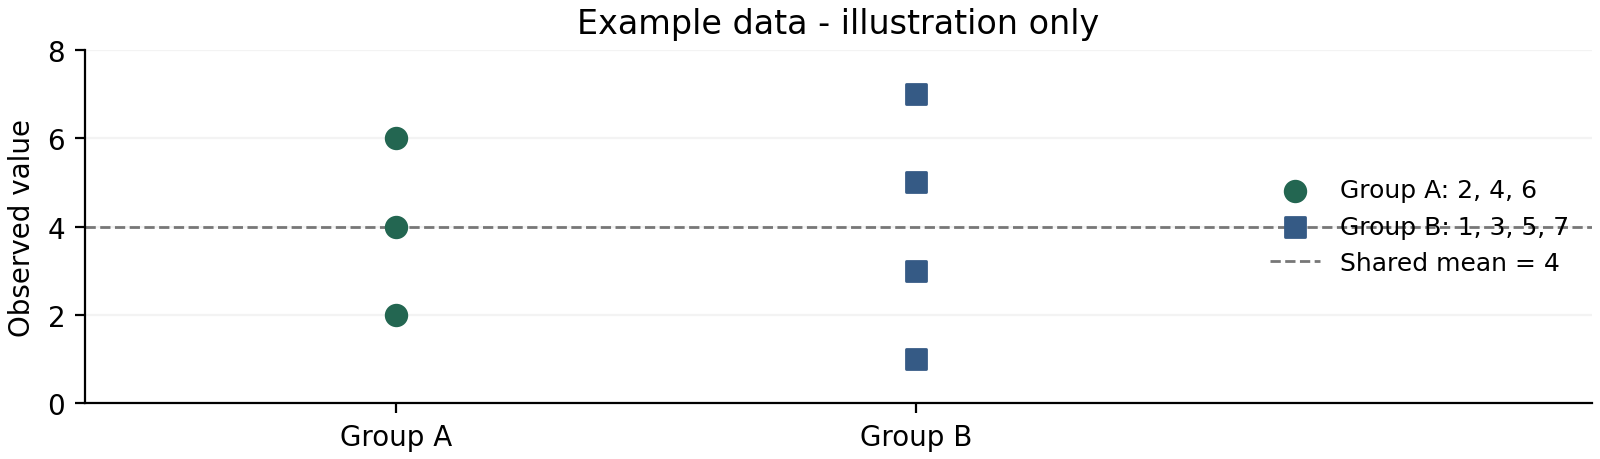
\includegraphics[width=0.9\linewidth]{figures/example-results.png}
  \caption{示例图片：两组演示数据的观测值与均值（请替换为自己的图片）}
  \label{fig:workflow}
\end{figure}

图~\ref{fig:workflow}~是一张实际插入的示例图片。两组数据均值相同，但其分布可能不同；
实际分析还应报告离散程度。这里的数据仅用于展示作业排版，不代表实证研究结果。
\end{solution}
